\documentclass[a4paper, 12pt]{article}

\usepackage{amsmath, amsthm, amssymb, graphicx}

\newtheorem{theorem}{Theorem}


\begin{document}

\title{An Introduction To \LaTeX}
\author{Rohan Alexander\\
\textit{Australian National University}}
\date{14 September, 2017}
\maketitle


\begin{abstract}
The point of this document is to introduce you to \LaTeX. There are many examples that you can grab and use in your own work.
\end{abstract}


\section{Introduction}
My father's father was a Methodist minister. He was a tall, handsome, noble-looking man; he had a deep beautiful voice. My father was an ardent atheist and admirer of Clarence Darrow. He skipped grades the way other boys skip class, he lectured my grandfather's flock on carbon 14 and the origin of species, and he won a full scholarship to Harvard at the age of 15.

He took the letter from Harvard to his father.

Something looked through my grandfather's beautiful eyes. Something spoke with his beautiful voice, and it said: It's only fair to give the other side a chance \cite{DeWitt2000}. 


\section{Model}
Using $\alpha$ to indicate the outcome of interest, the estimate becomes :
$$ \hat{\alpha} = \frac{\sum^J_{j=1}\beta_j}{\int^{\infty}_{0}f(k)} $$

And when $\lim_{k\rightarrow0}f(k)/k = \infty$ it is the case that $\int^{\infty}_{0}f(k) = 100$.

Often we care about probability, $\mathbb{P}$, because of expectations, $\mathbb{E}$, over real numbers $\mathbb{R}$.

It can be surprising when you first learn that $\frac{\frac{x}{y}}{y} = \frac{x}{y^2}$.

\begin{theorem}
Often we want to construct and prove theorems in economics.
\end{theorem}
\begin{proof}
My proof of the proposition.
\end{proof}


\section{Data}
Our datasets were downloaded from:
\begin{itemize}
\item the ABS; and
\item the RBA.
\end{itemize}

We had two priorities:
\begin{enumerate}
\item reproducibility; and
\item ease of use.
\end{enumerate}

\begin{tabular}{ l | c || r }
  \hline
  1 & 2 & 3 \\
  4 & 5 & 6 \\
  7 & 8 & 9 \\
  \hline  
\end{tabular}
  
\begin{figure}[h!]
\caption{My first image}
\center
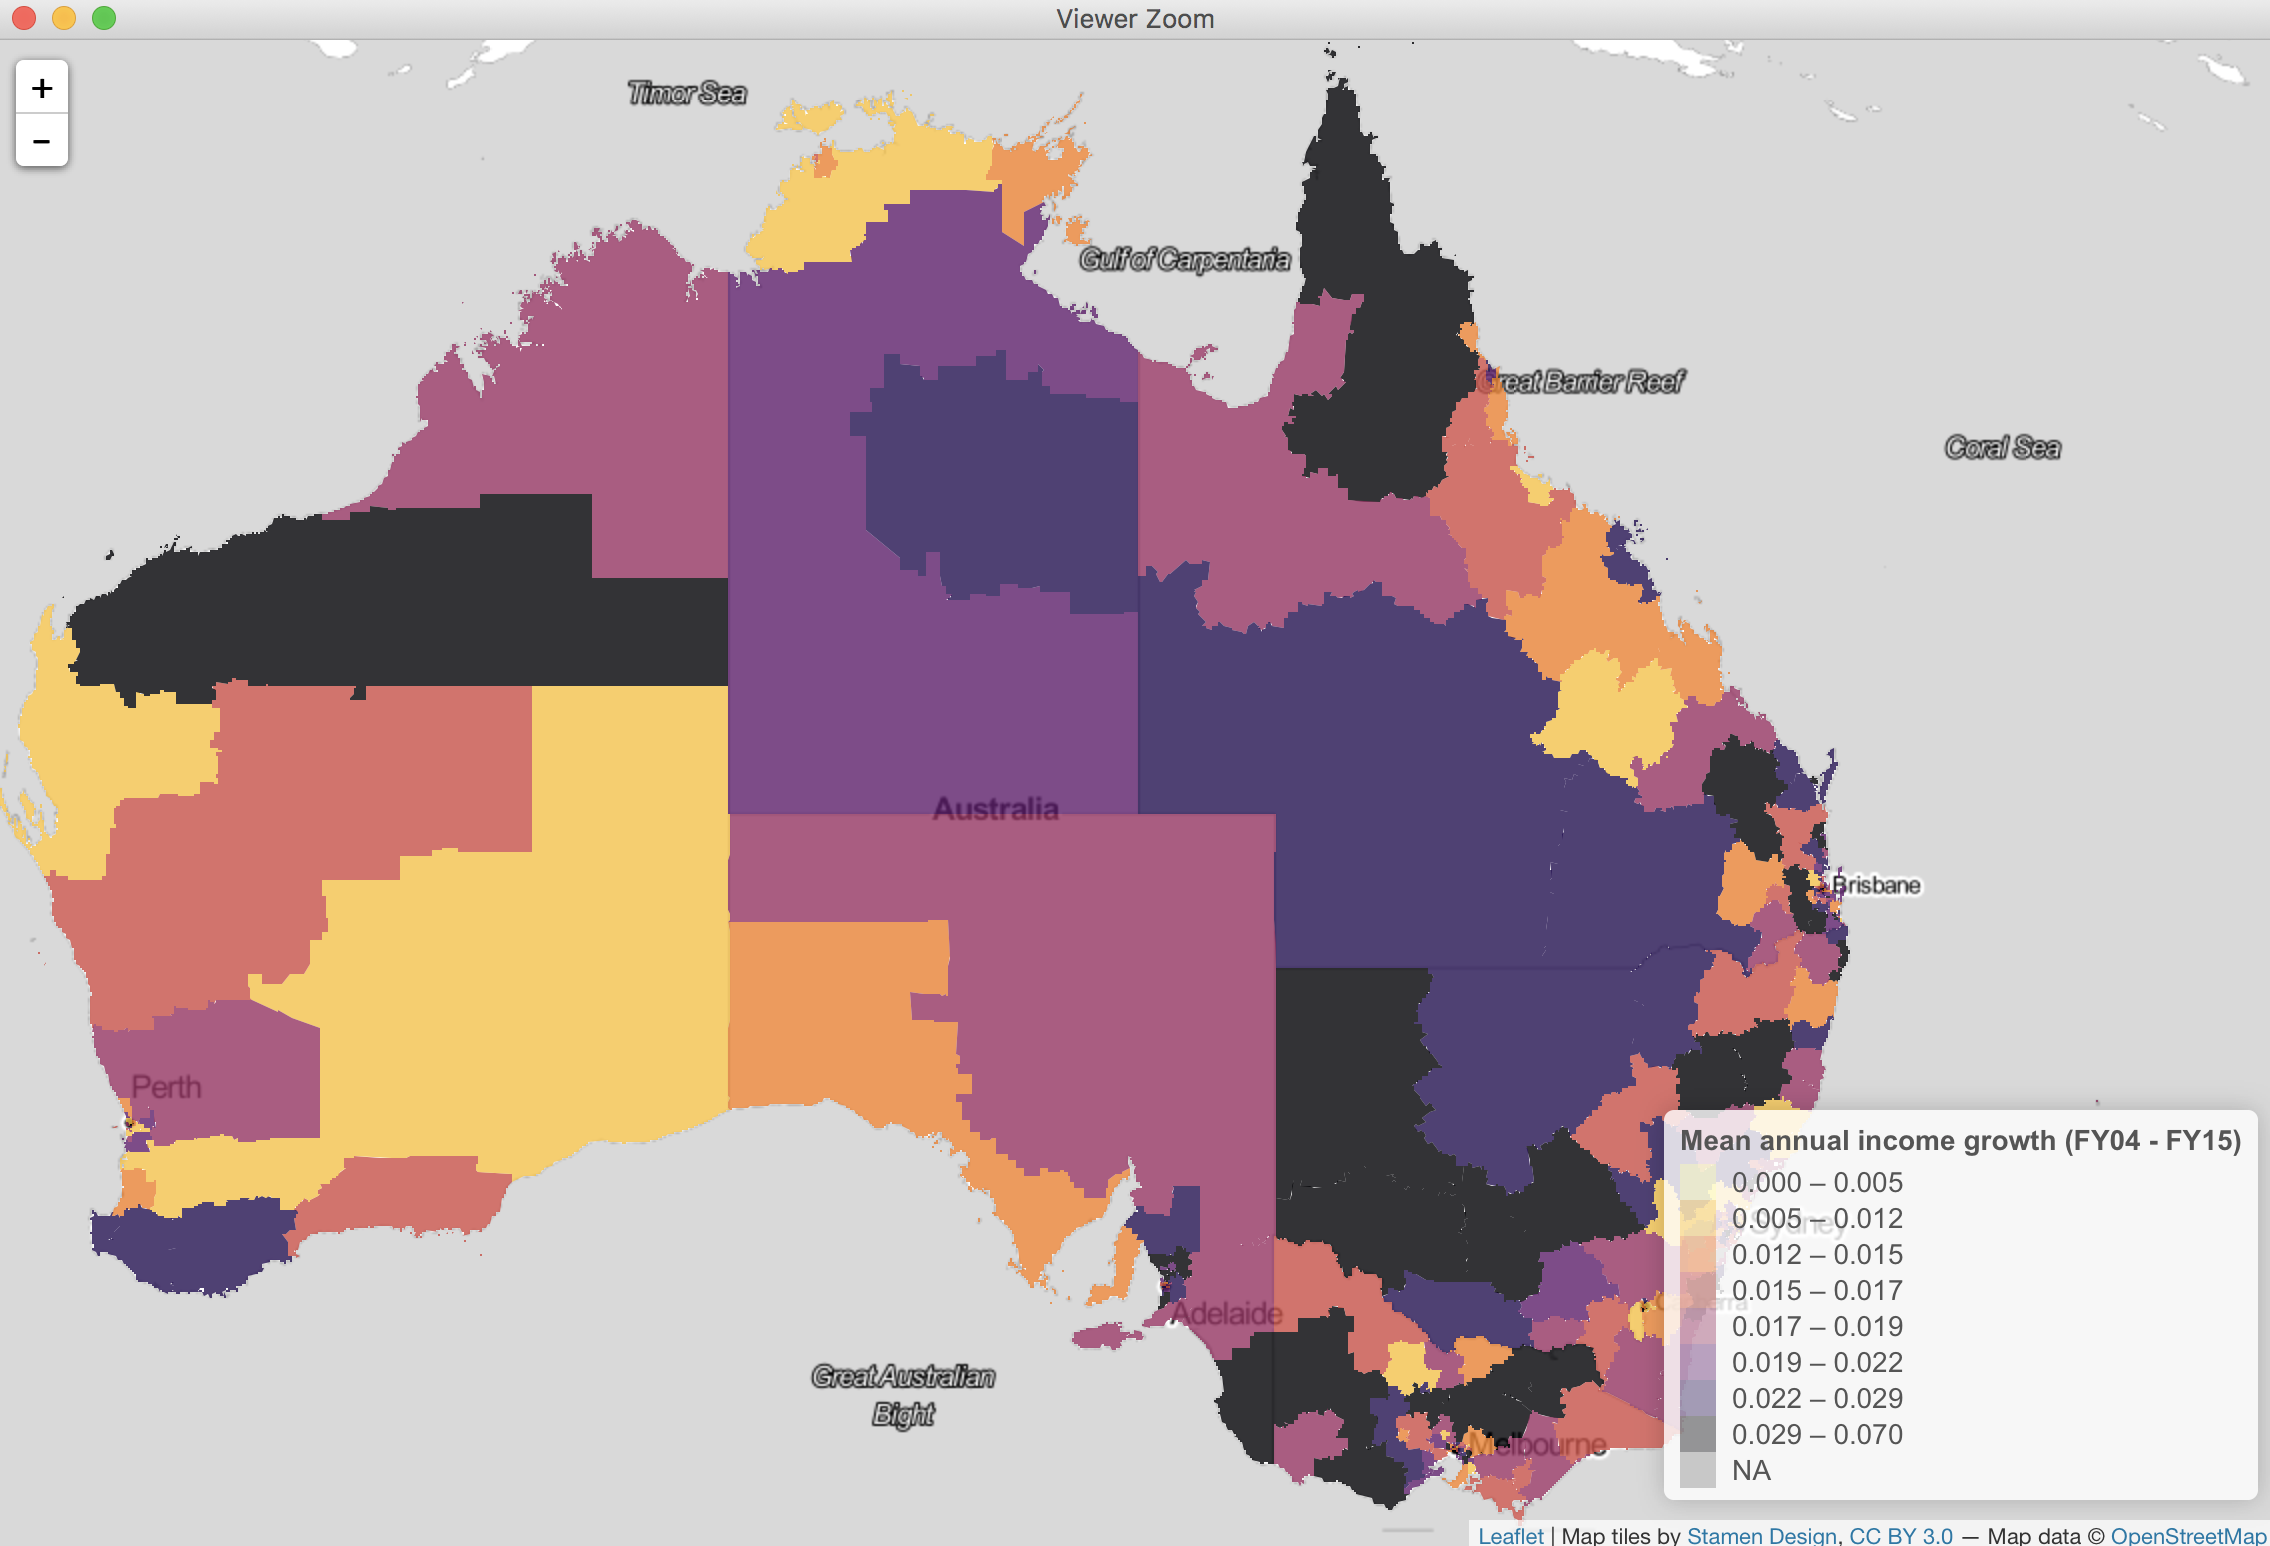
\includegraphics[width=0.80\textwidth]{me.png}\label{australia_map}
\end{figure}

Income inequality in Australia is illustrated in Figure \ref{australia_map}.

\bibliographystyle{apalike}
\bibliography{first_bibliography.bib}


\end{document}
